\documentclass[11pt,letterpaper]{article}

% Main document
% !TEX root = main.tex
\usepackage[margin=1in]{geometry}
\usepackage{amsmath}
\usepackage{amssymb}
\usepackage{graphicx}
\usepackage{hyperref}
\usepackage[backend=biber,style=numeric]{biblatex}
\addbibresource{bibliography.bib}
\title{From Tunneling Junctions to Continuum Response: A Physics-Informed Computational Model for Strain-Dependent Conductivity in Piezoresistive Systems}
\author{Shah Yusuf Safi}
\date{\today}

\input{preamble.tex}

\begin{document}
\maketitle

\begin{abstract}
    Many sensing devices rely on transduction mechanisms that convert mechanical deformation into measurable electrical signals. 
One important example is the piezoresistive effect, in which the electrical conductivity of a material varies with mechanical strain. 
This coupling between mechanical deformation and electrical conduction provides a natural setting for the study of multiphysics systems.

    This thesis develops a mathematical model describing conductive materials whose electrical conductivity depends on the underlying mechanical strain field. 
The mechanical behavior is described by the equations of elasticity, while the electrical potential satisfies a conductivity equation with strain-dependent coefficients. 
The resulting formulation leads to a nonlinear coupled system of partial differential equations of the form

\[
\nabla \cdot \boldsymbol{\sigma}(u) = 0, \qquad
\nabla \cdot (\sigma(\varepsilon(u)) \nabla V) = 0,
\]

where $ u $ denotes the displacement field, $ V $ the electrical potential, and the conductivity coefficient depends on the strain tensor $ \varepsilon(u) $.

    The primary objective of this work is to investigate this coupled electromechanical system from a computational modeling perspective. Emphasis is placed on the formulation and
analysis of the underlying multiphysics model, as well as on the development of computational strategies for approximating its solutions. In addition to classical numerical techniques, 
the study explores hybrid approaches that combine physics-based modeling with data-driven approximation methods to represent complex strain–conductivity relationships.

    The proposed framework aims to provide insight into strain-dependent electrical behavior in deformable media and contributes to the broader study of nonlinear 
multiphysics PDE systems arising in sensing and material modeling.

The results of this study are expected to provide insight into strain-dependent electrical behavior in deformable materials and contribute to the design and analysis of piezoresistive 
systems. Potential applications include structural health monitoring, wearable electronics, and soft robotics.

\end{abstract}

\tableofcontents

% Sections
% ================================
% INTRODUCTION
% ================================
\section{Introduction}
\label{sec:introduction}

The piezoresistive effect arises from the coupling between mechanical deformation 
and electrical conduction. In typical applications, a doped semiconductor element 
(such as silicon) is embedded within a mechanical structure, where external forces 
induce strain in the material. This deformation alters the electronic transport properties 
of the material, leading to measurable changes in its electrical response, commonly observed 
as variations in voltage or resistance.

\begin{figure}[htbp]
    \centering
    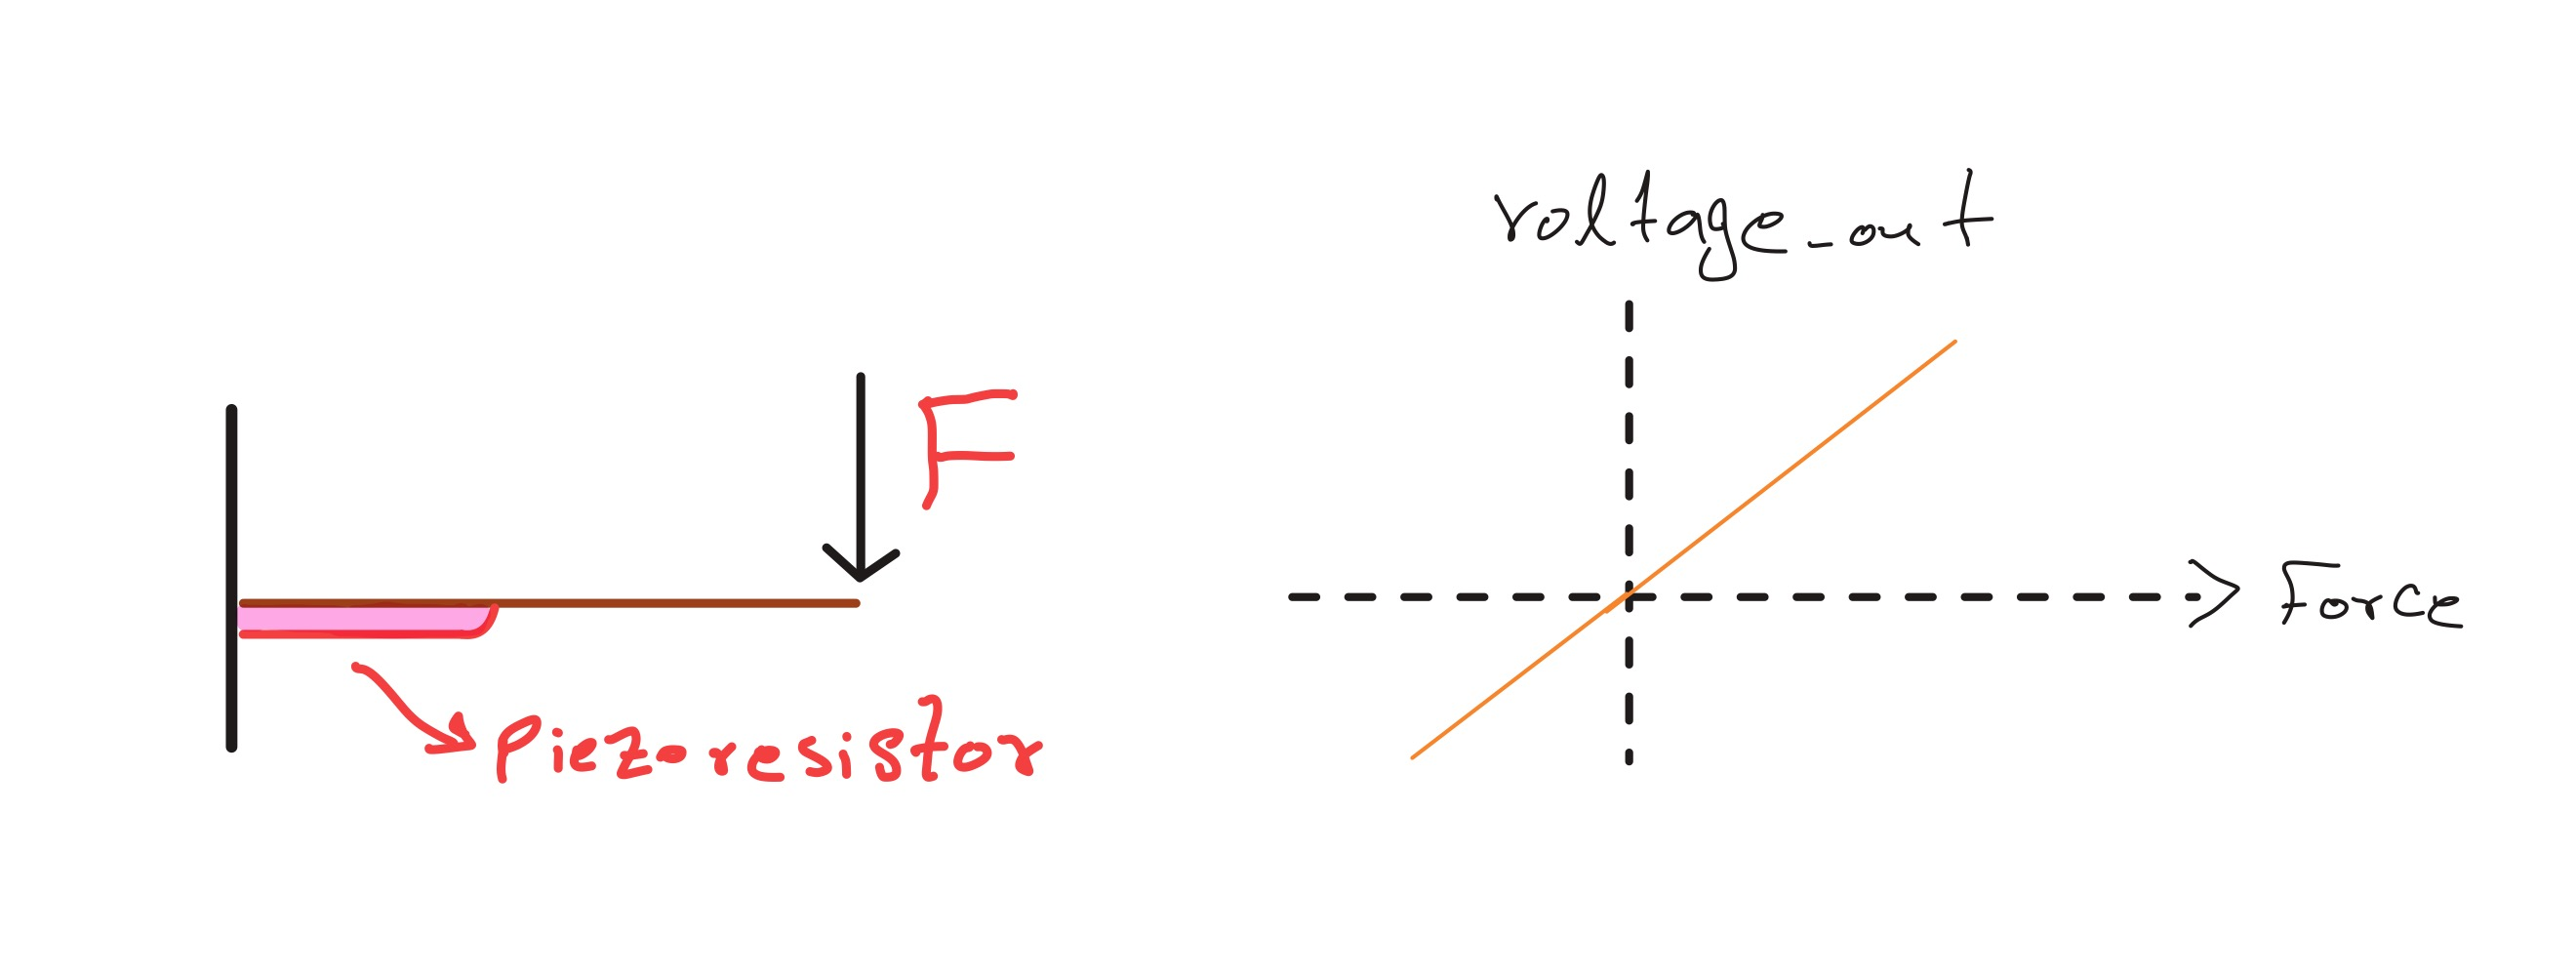
\includegraphics[width=0.5\textwidth]{Images/phenomenon.jpeg}
    \caption{A schematic representation of the piezoresistive effect, where mechanical deformation leads to changes in electrical response.}
\end{figure}

The piezoresistive effect, first observed by William Thomson (Lord Kelvin) 
in the 19th century and later developed for semiconductors by Bardeen, Shockley, and Smith \cite{smith1954}, 
describes the dependence of electrical conductivity on mechanical deformation. 
At a microscopic level, this behavior can be attributed to changes in the electronic structure 
and carrier transport mechanisms induced by strain, which modify quantities such as mobility 
and effective mass.

There exists a wide spectrum of engineering realizations of the piezoresistive effect, 
including strain gauges, pressure sensors, microelectromechanical systems (MEMS), 
cantilever-based sensing devices, and flexible or wearable systems \cite{doll2013}. 
Although these systems differ in geometry, material composition, and boundary conditions, 
they share a common physical origin rooted in the interaction between mechanical deformation 
and electronic transport.

Despite extensive technological development and optimization, the modeling of this coupling 
is often performed in a phenomenological and application-specific manner, where the dependence 
of conductivity on strain is introduced empirically. From a computational materials perspective, 
this raises the question of how such macroscopic descriptions can be related to the underlying 
physical mechanisms governing charge transport.

This work aims to address this by developing a computational framework that captures the 
electromechanical coupling at the continuum level, while maintaining a clear connection to the 
underlying physical processes. In this context, the continuum model serves as an effective 
description of strain-dependent conductivity, providing a bridge between microscopic transport 
phenomena and macroscopic device behavior.


\section{Problem Statement and Motivation}

Consider a conductive element with length $L$, cross-sectional area $A$, and resistivity $\rho$. 
Its electrical resistance is given by

\begin{equation}
    R = \frac{\rho L}{A}.
\end{equation}

Under mechanical loading, both geometry and material properties change. In particular, 
the length, area, and resistivity become functions of deformation, making resistance 
dependent on the mechanical state.

Using Ohm's law,

\begin{equation}
    R = \frac{V}{I},
\end{equation}

and expressing voltage and current as

\begin{equation}
    V = EL, \qquad I = JA,
\end{equation}

we obtain

\begin{equation}
    \frac{EL}{JA} = \frac{\rho L}{A}.
\end{equation}

Canceling geometric terms yields the local relation

\begin{equation}
    \mathbf{J} = \sigma \mathbf{E}, \qquad \sigma = \frac{1}{\rho},
\end{equation}

where $\mathbf{E} = -\nabla V$.

Combining this with charge conservation in steady state,

\begin{equation}
    \nabla \cdot \mathbf{J} = 0,
\end{equation}

leads to the conductivity equation

\begin{equation}
    \nabla \cdot (\sigma \nabla V) = 0.
\end{equation}

The resulting equation is an elliptic PDE in divergence form, belonging to a well-studied class 
of second-order equations in the theory of partial differential equations \cite{evans}.

In piezoresistive materials, the conductivity depends on strain:

\begin{equation}
    \sigma = \sigma(\varepsilon(u)),
\end{equation}

where the strain tensor is given by\footnote{The strain tensor is defined as the symmetric part of the displacement gradient, which removes rigid body rotations and captures the true deformation of the material.}

\begin{equation}
    \varepsilon(u) = \frac{1}{2}(\nabla u + \nabla u^T).
\end{equation}

This introduces a nonlinear coupling between mechanical deformation and electrical conduction.


\begin{figure}[htbp]
    \centering
    
\includegraphics[width=0.7\textwidth]{images/model1.png}
    \caption{Change of geometric and material properties under mechanical deformation. $L$ denotes the length of the conductor, $W$ its characteristic width, 
and $A = W^2$ the cross-sectional area (assuming a square cross-section). 
The material property $\rho$ represents the electrical resistivity, which may vary under mechanical deformation.
    Both the dimensions and the resistivity of the conductor vary, leading to a strain-dependent resistance.}
\end{figure}

This illustrates that both geometric deformation and intrinsic material changes contribute to the variation of resistance.

\section{Mathematical Model}

Based on the physical considerations discussed above, the coupled electromechanical behavior 
can be described at the continuum level by a system of partial differential equations.

The mechanical response of the material is governed by the equations of elasticity,

\begin{equation}
    \nabla \cdot \boldsymbol{\sigma}(u) = 0,
\end{equation}

where $u$ denotes the displacement field and $\boldsymbol{\sigma}(u)$ is the stress tensor, 
which depends on the strain.

The electrical response is described by the conductivity equation,

\begin{equation}
    \nabla \cdot \left( \sigma(\varepsilon(u)) \nabla V \right) = 0,
\end{equation}

where $V$ is the electrical potential and the conductivity $\sigma$ depends on the strain tensor 
$\varepsilon(u)$.

Together, these equations define a coupled system in which mechanical deformation influences 
electrical conduction through the strain-dependent conductivity. From a physical perspective, 
this coupling represents an effective description of how deformation alters the underlying 
electronic transport properties of the material.

This formulation provides the basis for computational modeling of the piezoresistive effect 
within a continuum framework.

\section{State of Research}

The piezoresistive effect has been extensively investigated in both experimental and engineering contexts, 
particularly in the development of semiconductor-based sensors and microelectromechanical systems (MEMS) \cite{smith1954,doll2013}. 
Early studies established the strong dependence of electrical conductivity on mechanical strain in semiconductors such as silicon, 
highlighting the role of crystal structure and carrier transport in determining the sensitivity of the effect.

From a materials physics perspective, piezoresistivity originates from strain-induced modifications of the electronic structure 
and charge transport properties. In semiconductors, mechanical deformation can alter band structure, carrier mobility, and scattering mechanisms, 
leading to significant changes in conductivity. These effects have been studied using both phenomenological models and more detailed 
electronic transport theories.

In practical applications, however, the coupling between mechanical deformation and electrical response is often modeled in a simplified 
and application-specific manner, where the dependence of conductivity on strain is introduced empirically. While such approaches are effective 
for device design and optimization, they do not always provide a transparent connection between the underlying physical mechanisms and the 
resulting macroscopic behavior.

At the continuum level, models based on partial differential equations are widely used to describe both elasticity and electrical conduction. 
However, the integration of strain-dependent transport properties into such models is typically treated in a phenomenological way, and a 
systematic computational framework that bridges physical insight and continuum modeling remains an open challenge.

Such a framework is particularly relevant for understanding emerging materials and 
devices where electromechanical coupling plays a central role.

Based on these considerations, the proposed study is guided by the following research questions:

\begin{itemize}
    \item How can strain-dependent conductivity be incorporated into a consistent continuum model of electromechanical coupling?
    \item How does mechanical deformation influence the spatial distribution of electrical potential in conductive materials?
    \item What qualitative and quantitative effects arise from the nonlinear coupling between mechanics and electrical transport?
    \item To what extent can flexible (e.g. data-driven or physics-informed) approaches improve the modeling of $\sigma(\varepsilon)$?
\end{itemize}

To address these questions, the research will be structured around the following key components:

\begin{itemize}
    \item Physical background and modeling assumptions
    \item Formulation of the coupled electromechanical model
    \item Analysis of the nonlinear system
    \item Computational methods and numerical experiments
    \item Interpretation of results in the context of material behavior
\end{itemize}



`\section{Methodology}

The proposed study follows a computational approach based on a continuum description of the coupled electromechanical system. 
The methodology is structured in several stages, combining physical modeling with numerical approximation.

First, the governing equations of elasticity and electrical conduction are formulated within a consistent continuum framework. 
The mechanical problem provides the displacement field $u$, from which the strain tensor $\varepsilon(u)$ is computed. 
This strain field serves as input to the electrical problem through the strain-dependent conductivity $\sigma(\varepsilon)$.

As a baseline, the electrical conduction problem with constant conductivity is considered and solved numerically. 
This case admits an analytical solution and is used to validate the numerical implementation. 
A finite element discretization is employed to approximate the solution, and the numerical results are compared against the exact solution.

\begin{figure}[htbp]
    \centering
    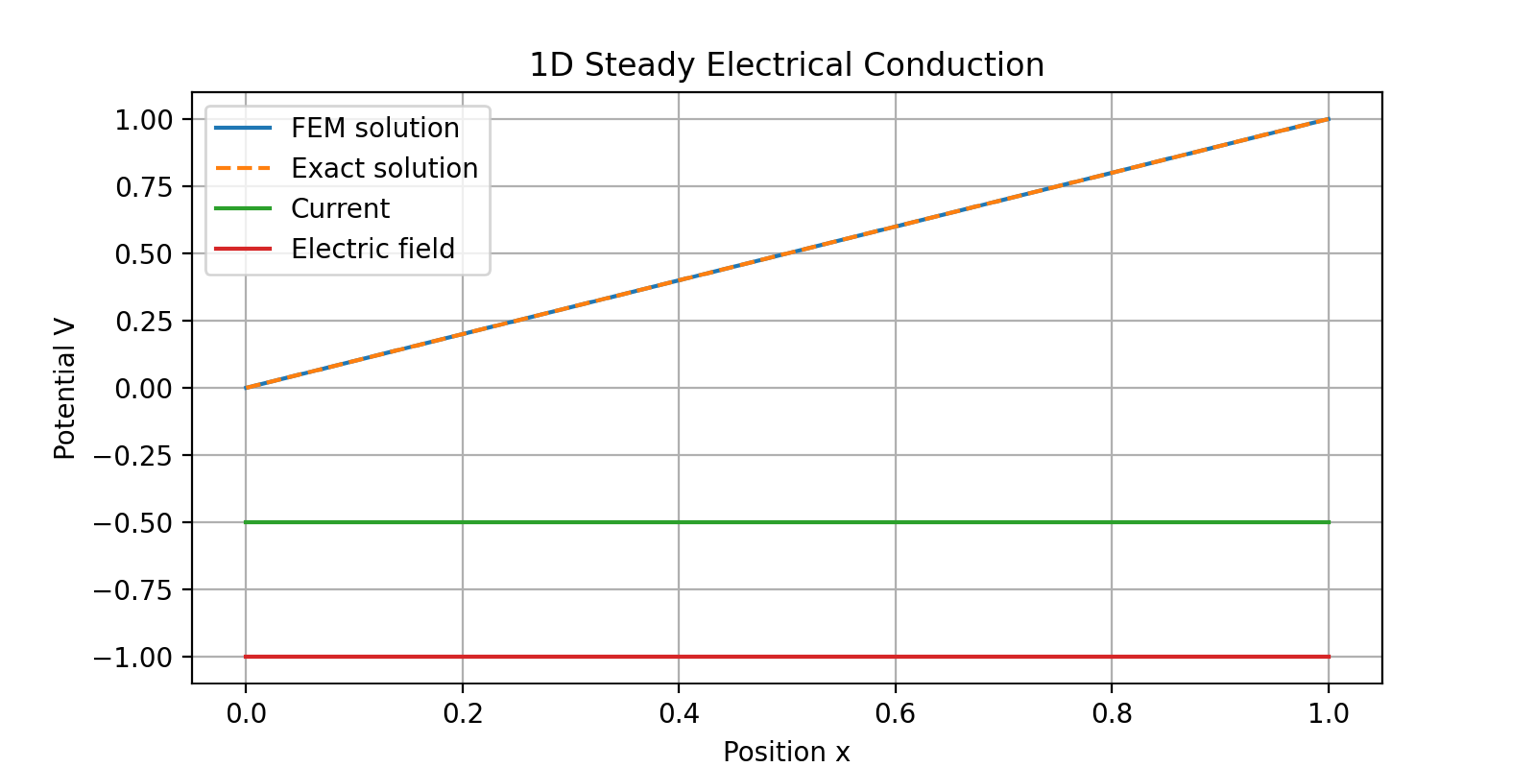
\includegraphics[width=0.75\textwidth]{Images/1d_cond.png}
    \caption{Finite element solution of the 1D steady conduction problem with constant conductivity compared with the analytical solution. 
    The linear potential profile and constant electric field confirm the expected physical behavior.}
\end{figure}

Building on this, the full coupled system is addressed by introducing a spatially varying conductivity $\sigma(\varepsilon(u))$. 
The problem is solved iteratively: the mechanical and electrical fields are updated in a coupled manner until convergence is achieved. 
Special attention is given to the nonlinear nature of the coupling, which may lead to non-uniform fields and sensitivity to deformation.

From a computational perspective, the finite element method (FEM) is used as the primary discretization technique due to its flexibility in handling 
heterogeneous material properties and complex geometries. The implementation focuses on robustness and clarity, enabling systematic exploration 
of different forms of the strain–conductivity relation.

In addition, the methodology allows for extensions beyond purely phenomenological models. 
In particular, the constitutive relation $\sigma(\varepsilon)$ can be treated as a flexible component, 
which may be informed by physical insight or approximated using data-driven approaches. 
This provides a pathway to incorporate more detailed transport behavior without modifying the overall computational framework.

Overall, the methodology is designed to provide a transparent and extensible computational pipeline, 
bridging continuum modeling with physically motivated descriptions of strain-dependent conductivity.'




\section{Expected Outcome}

The expected outcome is a computational framework for analyzing strain-dependent electrical conduction.

The model will provide insight into how deformation affects electrical response and sensitivity.

From a broader perspective, the work contributes to the study of nonlinear multiphysics PDE systems 
and may support applications in sensing, materials modeling, and structural monitoring.



\clearpage
\printbibliography

\end{document}
